\documentclass[11pt,letterpaper,final]{article}

% font/type display packages
\usepackage{amsmath}
\usepackage{amsfonts}
\usepackage{amssymb}
\usepackage{type1cm}
\usepackage{palatino} \linespread{1.05}
\usepackage{courier}
\usepackage{relsize}

% packages for floats, figures, tables, boxes etc.
\usepackage{float}
\usepackage{flafter}
\usepackage{graphicx}
\usepackage{tabularx}

% caption package must go after float, rotate, and subfigure, [hang]
\usepackage[sc,bf,small]{caption}
\usepackage{setspace}
\usepackage{hyphenat}
\usepackage{fancyhdr,lastpage}

\usepackage{booktabs}
\usepackage{endnotes}
\usepackage{ulem}

\usepackage[table]{xcolor} % For row colors

\usepackage[at]{easylist}
	\makeatletter
	\newcommand{\el@aux}[1]{\vspace*{.3\baselineskip}\begin{easylist}[itemize]\ListProperties(Style*=--\hskip .5em)  #1 \end{easylist}\vspace*{.3\baselineskip}\endgroup}
	\newcommand{\el}{\begingroup\Activate\el@aux}
	\makeatletter

% url allows for formatted urls with linebreaks
\usepackage{hyperref}
\hypersetup{
    bookmarks=true,         % show bookmarks bar?
    unicode=false,          % non-Latin characters in Acrobat’s bookmarks
    pdftoolbar=true,        % show Acrobat’s toolbar?
    pdfmenubar=true,        % show Acrobat’s menu?
    pdffitwindow=false,     % window fit to page when opened
    pdfstartview={FitH},    % fits the width of the page to the window
    pdftitle={My title},    % title
    pdfauthor={Author},     % author
    pdfsubject={Subject},   % subject of the document
    pdfcreator={Creator},   % creator of the document
    pdfproducer={Producer}, % producer of the document
    pdfkeywords={keyword1} {key2} {key3}, % list of keywords
    pdfnewwindow=true,      % links in new window
    colorlinks=false,       % false: boxed links; true: colored links
    linkcolor=red,          % color of internal links
    citecolor=green,        % color of links to bibliography
    filecolor=magenta,      % color of file links
    urlcolor=cyan           % color of external links
}
% packages for bibs and cites
	\usepackage{natbib}
	\usepackage{har2nat}
	\newcommand{\possessivecite}[1]{\citeauthor{#1}'s \citeyearpar{#1}}
	\usepackage{breakcites}

%Change page geometry for dissertation
\usepackage[top=1in, bottom=1in, left=1in, right=1in]{geometry}

\usepackage{geometry} % For margin adjustments

\geometry{
  left=25mm,
  right=25mm,
  top=25mm,
  bottom=25mm
}

%\usepackage[compact,tiny,sc,bf]{titlesec}
%\titlespacing{\section}{0pt}{\baselineskip}{*1}
%\titlespacing{\subsection}{0pt}{\baselineskip}{*1}
%\titlespacing{\subsubsection}{0pt}{\baselineskip}{*1}

% depth of section numbering
\setcounter{secnumdepth}{0}

% url style
\makeatletter
\def\url@leostyle{\@ifundefined{selectfont}{
\def\UrlFont{\sf}}{
\def\UrlFont{\smaller\ttfamily}}}
\makeatother\urlstyle{leo}

\usepackage{abbrevs}

% options for fancy headers and footers
  \pagestyle{fancy} \lhead{Urban Econ. Syllabus} \chead{} \rhead{\today} \lfoot{} \cfoot{}
  \rfoot{\thepage /\pageref{LastPage}}
  \renewcommand{\headrulewidth}{0pt}
  \renewcommand{\footrulewidth}{0pt}
  
\usepackage{multicol}

\begin{document} \singlespacing

%\thispagestyle{empty}
\begin{center}
	{\bf\scshape\LARGE Urban Economics \\Syllabus\\} \normalsize
ECON 3320-01 \\ 
3 credit hours \\
Fall 2021\\
TTH 11:00 \AM-12:15\PM\ in Tilton Hall 301
\end{center}


\begin{tabbing}
	Instructor: \hspace{0.5cm} \= Professor Hussain Hadah \\ \kill 
	\> Department of Economics\\
	\> School of Liberal Arts \\
	\> Tulane University\\
		Pronouns: \> He/Him (\href{https://www.mypronouns.org/}{What's this?}) \\
	Office hours: \> By appointment using \href{https://hussainhadah.youcanbook.me/}{https://hussainhadah.youcanbook.me/} \\
	Email: \> \href{mailto:hhadah@tulane.edu}{hhadah@tulane.edu}\\
		Room: \> Tilton Memorial Hall Room 103\\
    % Time: \\
\end{tabbing}

\begin{multicols}{2}
  \tableofcontents
\end{multicols}

\newpage

\section{Catalog/Course Description}
A review of the determinants of the location, size, growth, and form of urban areas. Study of the major issues of contemporary urban life: physical deterioration, growth of ghettos, congestion, pollution, transportation, and land use.

\subsection{A More Detailed/Updated Course Description}
The field of urban economics addresses a wide variety of questions and topics. At the most general level, the field introduces space into economic models and studies the location of economic activity. Urban economics incorporates a lot of topics that also overlap with other fields, but the topics have a spatial or regional element. For example, the economics of crime overlaps with labor economics, since labor economics typically discusses the choice to work or not work, but because crime is thought of as a local phenomenon, it also falls under urban economics. Similarly, local government finance falls under both public economics (since that field deals with government) but also urban economics due to the local nature of the government. 

Given how broad the field of urban economics is, this course focuses on the following urban economics topics: geographical data, agglomeration economies and the economics of cities, economic development and tax incentives, crime, gender-based violence, housing and housing policy, neighborhood effects, and transportation. 

My course covers both the theoretical (applications of mathematical models) and empirical research (statistical analysis) on urban economics about equally. Many instructors only cover theory, presenting mathematical models of the economy (often using graphs, because math is hard!) By empirical methods I mean that I will be teaching you at a very non-technical and intuitive level how economists use data to analyze urban economics questions. Essentially I will be teaching you applied econometrics without as many equations or statistical theory. The lessons will be very intuitive and more focused on how the methods are used in policy analysis. I will also teach you how to use geographical data from the Census using tools such as American Factfinder.

\subsection{Prerequisites}
The prerequisites for this course are introductory microeconomics (ECON 1010) and high school-level algebra (e.g., solve for X, graph a line) and high-school level statistics (e.g., calculating medians, ideally remembering the basics of hypothesis testing.) 

Unofficially, familiarity with statistics and econometrics will be helpful. For example, knowing what a standard error is and what confidence intervals are would be ideal. Understanding the basics of linear regression will also help a lot. Most students can easily handle the course material since I handle statistics in a more intuitive way, but more background always helps.

\section{Course Objectives} 
This course provides an introduction to urban economics. Topics include the economics of cities, local and regional economic development, using geographic data, housing markets and housing policy, and crime.

\section{Course Learning Objectives} The learning outcomes below list many of what I hope students will grasp after this course. This is a non-exhaustive list and it may change over time. 

After completing this course, students will be able to...
\el{
@ \textbf{Geographical Data}
@@ Explain how the U.S. Census defines regions (e.g., CBSA, MSA)
@@ List census geographies by size (i.e. region to Census Block)
@@ Describe the type of data on American FactFinder
@@ Select data on American FactFinder by level of geography
@@ Select from different topics on American FactFinder
@@ Create maps on American FactFinder
@@ Download data from American FactFinder as a spreadsheet

@ \textbf{Agglomeration and Clusters}
@@ Define urban agglomeration and be able to explain it intuitively to a non-economist.
@@ Discuss and evaluate at least three factors that can lead to urban agglomeration.
@@ Discuss the positive spillover effects from agglomeration.
@@ Identify urban amenities that lead to agglomeration economies.
@@ Summarize the effect of agglomeration on at least one industry (e.g., entertainment, technology).
@@ Discuss at least two regional clusters (e.g., Silicon Valley, Route 128, the ``Hollywood" film industry, Detroit's Auto Industry).
@@ Evaluate the likely impact of agglomeration on particular firms of industries.
@@ Use the online tools on clustermapping.us to find data on how industries are distributed geographically, and find data on the industry mix within particular regions.

@ \textbf{Urban and Regional Economic Development}
@@ Explain both graphically and intuitively the effects of economic development on labor and land markets.
@@ Argue who is more likely to benefit (or not) from economic development.
@@ Discuss the extent to which tax rates and subsidies could be used to increase economic development.
@@ Evaluate which factors affect the location of firms.
@@ Discuss at least three papers that studied the effect of tax incentives on firm location or economic development.
@@ Argue using evidence what the effect of tax incentives on firm location and economic development is.
@@ Discuss what factors might make tax incentives more influential for firm location, or less influential.
@@ Discuss the effects of at least two of the following incentives: film incentives, biotech incentives, and enterprise zones.

@ \textbf{Crime}
@@ Use the ``rational criminal" model to predict how certain events (e.g., increase in inequality) may affect crime.
@@ Argue why the efficient level of crime is not zero in this model.
@@ Discuss to what extent this model played out in practice in different readings (e.g., \citep{Yang2017a})
@@ Explain why it is difficult to measure the impact of police on crime.
@@ Contrast at least three crafty ways that economists have tried to estimate the effect of police on crime given the issue of endogeneity.
@@ Explain implicit bias
@@ Discuss research on to what extent implicit bias affects decisions in policing and in the criminal justice system, synthesizing this research into your own position and narrative.
@@ Discuss research and come to conclusions on the extent to which there is racial bias in policing and criminal justice outcomes
@@ Explain what the ``ban the box'' movement is and the implications of not letting employers ask about applicants' criminal histories.
@@ Discuss the implication of ``ban the box'', especially by race and ethnicity.
@@ Apply economics research to questions motivated by the Black Lives Matter movement, such as if racial bias exists, if police disproportionately apply force to minorities, if defunding the police is a good idea, and what policy approaches exist to help solve the issues we face.

@ \textbf{Gender-Based Violence Module}
@@ State the general incidence of gender-based violence in the US.
@@ Recall some definitions and terminology around gender-based violence.
@@ Summarize research on the different impacts of gender-based violence on individuals and on society more broadly. 
@@ Summarize how COVID-19 has affected gender-based violence.
@@ Describe how economic tools, such as a difference-in-differences, can be used to study gender-based violence.

@ \textbf{Housing Policy}
@@ Provide examples of housing policies that range from financial incentives to regulations.
@@ Evaluate policies designed to make housing more affordable or accessible.
@@ Apply the basic supply-and-demand (perfect competition) model to predict the effects of rent control on the housing market.
@@ Evaluate the applicability of the basic supply-and-demand (perfect competition) model relative to other models of the housing market.
@@ Recite some empirical evidence on the effects of rent control on housing markets.
@@ Provide an example of how economists have studied homelessness.
@@ Provide an example of how economists have studied evictions.
@@ Summarize how eviction rates and policy have changed due to COVID-19.

@ \textbf{Neighborhood Effects and Housing Vouchers}
@@ Describe at least three effects that neighborhoods can have on the socio-economic outcomes of individuals and/or families.
@@ Provide at least one example of how researchers have tried to estimate the effect of neighborhoods while controlling for the self-selection of individuals and families into neighborhoods.
@@ Critique the Moving to Opportunity program.
@@ Discuss what ``Neighborhood effects'' are.
@@ Discuss how it is difficult to measure the effects of neighborhoods or the value of the good neighborhoods.
@@ Explain to a parental figure how the Moving to Opportunity program worked.
@@ Argue why an experiment was necessary to measure the causal effect of neighborhoods in this case.
@@ Explain what problems occur given that not everyone accepts ``treatment'' in an experiment.
@@ Explain what ``Intent to Treat'' means in the context of an experiment.
@@ Contrast different types of voucher policies and to what extent they affect socio-economic outcomes, according to research.

@ \textbf{Transportation}
@@ Summarize research on the effects of ride-sharing expansions on policy outcomes (e.g., alcohol-related traffic fatalities).
@@ Describe how and to what extent economists and social scientists can isolate the effects of ridesharing on policy outcomes using a difference-in-differences approach.

@ \textbf{Student Learning Outcomes that are not Topic-Specific}
@@ Explain the concepts of a confidence interval and ``statistically significant'' intuitively.
@@ Determine from reading published tables what estimates are statistically significant.
@@ Calculate a 95\% confidence interval from reading a point estimate and standard error from a table.
@@ Explain the intuitive idea behind difference-in-differences.
@@ Explain how difference-in-differences provides more causal estimates of the effects of policies compared to cross-sectional comparisons.
@@ Explain how differences-in-differences is used in at least one urban economics research paper.
@@ Evaluate the validity of a particular difference-in-differences approach in a research paper.
@@ Locate and download economic and demographic data at different regional levels (e.g., ZIP, county/parish) using the American Community Survey.
@@ Calculate basic statistics using geographical data.
@@ Locate peer-reviewed research using Google Scholar.
@@ Create reference section and add in-text citations in APA or Chicago Author-Year format.
@@ Use Google Scholar to get APA citations.
@@ Identify at least two peer-reviewed journals that publish urban economics research.
@@ Explain the difference between an endogenous variable and an exogenous variable and give an example of each from one model discussed in class.
@@ Discuss how COVID-19 affects the study of urban economics, such as which topics are important to study, or which urban economics phenomena are occurring.
}

\section{Program-Level Outcomes} This course contributes to economics major/minor by filling one of the elective requirements. This course also contributes to the major/minor by teaching students how to use/interpret the tools of microeconomics (theory, empirical methods) to explain topics in urban economics. 

The course is also useful to urban studies students who wish to learn economic approaches to analyzing urban issues. This course also contributes to the over-arching goal of ensuring that social science students are comfortable working with data.

\section{Core Curriculum Outcomes} Under the core requirements, required of all undergraduate students regardless of school/major, this course can satisfy both the ``Social \& Behavioral Sciences'' requirement and/or the ``Race \& Inclusion'' requirement.

\section{Required Student Resources}
The textbook for this course is
\begin{quote}
	Brueckner, Jan. 2011. {\em Lectures on Urban Economics}. Cambridge: MIT University Press.
\end{quote}
\nocite{Brueckner2011}

This textbook is available at the bookstore and is relatively cheap compared to other textbooks. In addition to the textbook, there will be several other readings, all of which will be available through Canvas. Roughly half of the course follows this textbook and the other half follows other readings or my own lecture material.

I will give announcements either via email and/or in class about upcoming readings and advice on what to focus on. Some of the readings are technical pieces from economics journals. The degree to which you to be familiar with the details of a paper will be clear from the emphasis given to the paper in lecture or will be clear based on instructions I give you. See more discussion of this later in the syllabus. 

It is your responsibility to follow my announcements and do the readings. Not keeping up to date on readings will negatively affect your ability to achieve the course learning objectives and will negatively affect your grade. For example, many classroom activities may require that you have read the readings before class.

\section{Evaluation Procedures and Grading} Success at achieving the learning outcomes above is measured through various course assignments. Your final course grade is based on the following breakdown:

\el{
@ Quizzes (Best \textbf{3} out of \textbf{4} x 20\% = 60\%)
@ Group Briefing Notes (Best \textbf{2} out of \textbf{3} x 10\% = 20\%)
@ Other Activities (20\%) (Three activities dropped)
}

In determining your final letter grade, I will first calculate a percentage grade based on the above criteria. Then I will convert this final percentage grade to a final letter grade as follows:

\el{
@ A = 93\% to 100\%, A- = 90\% to 92.99\%,
@ B+ = 87\% to 89.99\%, B = 83\% to 86.99\%, B- = 80\% to 82.99\%,
@ C+ = 77\% to 79.99\%, C = 73\% to 76.99\%, C- = 70\% to 72.99\%,
@ D+ = 67\% to 69.99\%, D = 63\% to 66.99\%, D- = 60\% to 62.99\%,
@ F = 0\% to 59.99\%
}

Note that I do not round grades up if you are close to a cut-off or otherwise tweak grades (e.g., apply a curve). I would prefer not to add subjectivity into the process as this is not fair. Please do not ask me to do this.

Below are more details on each individual evaluation criteria.

\subsection{Quizzes}
There will be four quizzes, all conducted during class time, using the entire class time. These are scheduled for Feb. 8, Mar. 5, Mar. 28, and Apr. 25. While these are ``open book,'' meaning you can bring and use course notes, documents on your computer, books, etc., you cannot communicate or work with anyone else. You will complete the quizzes on a computer using Canvas. You can conduct the quiz on your laptop in the classroom or remotely in a place of your choosing. 

The quizzes will be approximately two or three short answer questions and zero to two multiple choice questions. 

I use your three best quizzes, which each provide 15\% of the total course grade, for a total of 45\%. This provides flexibility for those you have to miss a quiz due to illness or other circumstances - that quiz is simply dropped. However, I may be able to make arrangements for you to take the quiz slightly later depending on your circumstances, but you need to arrange this beforehand if at all possible. Note that since you can take your quizzes online through Canvas, you can take these even if you are in quarantine or off campus.


\subsection{Group Briefing Notes}
There will be \textbf{three} graded group briefing note assignments, but only your best \textbf{two} will be counted. The goal for these is that you will get practice with the following:
\begin{enumerate}
\item Concise writing.
\item Citing sources, and creating a references section in APA format or Chicago Author-Year format.
\item Doing a literature review using Google Scholar.
\item Reading and summarizing published economics journal articles.
\item Coming to reasonable conclusions based on your assessment of the research.
\end{enumerate}
How this will work is that you will form groups of three to five beforehand, or I will create groups randomly through a jigsaw activity. Your group will work, during class time, to write a one page briefing note, single-spaced, in a Google Doc or OneDrive document.

I will provide guidance for the content of each briefing note through handouts, provided to you on Canvas beforehand. Your briefing note will seek to quickly introduce the reader, who may not have an economics background, to the topic and to summarize what the research says about the topic. Briefing note topics will be:

\begin{enumerate}
\item To what extent do tax incentives encourage economic development?
\item Is there racial bias in policing and in the criminal justice system?
\item What are the impacts of rent control on housing markets?
\end{enumerate}

\subsubsection{Grading and Revising the Group Briefing Notes}
These briefing notes will be graded on a ten point rubric that will be provided to you. You will start working on the first draft in class and, if you don't finish it during class, then you can finish it on your own time later. You get one week to complete the group note, then one week after that to submit a revision.

I will then grade your first draft as if it is a final document, so that you know exactly where you stand with that draft. I will be grading it as if I am a picky bureaucrat, and this briefing note were actually to be used to brief, say, an important government official. Thus, first round grades will be lower, between 4/10 and 8/10 likely. 

However, this first round grade is only temporary. If you submitted this draft by the deadline (before the next class) then you get a chance to make revisions. You will have one week from when I first grade your briefing note to make any revisions. I will provide detailed feedback that will guide you towards revisions you can make. Most students make revisions that increase their scores by at least two points. When you submit your final version, please email me the link to the Google doc again and in the body of your email, summarize your changes so I can more easily identify them and reward you for them. 

If you failed to submit your first draft before the deadline (before the next class) then whenever you submit, I will grade it as the final version but you will not have the opportunity to resubmit. Note that incorrectly sharing the Google Doc with me could result in your assignment being late.

Students that miss day(s) when we do briefing notes will get a zero on that assignment unless they choose to do the briefing note on their own later (email me to make arrangements). However, to provide some additional flexibility, I drop your lowest briefing note grade. That is, I use your two best (out of three) scores. This policy is designed to accommodate students who cannot attend the course when we have a briefing note assignment.

\subsubsection{How to Properly Submit the Group Briefing Notes}
You will submit your group briefing notes on Canvas by submitting a link to the Google Doc or OneDrive document. Please ensure that the link you submit allows anyone with the link to edit the document. Confirm that the sharing settings for the URL allows anyone with the URL to access and edit the document. Other options (e.g., sharing the document with my Tulane.edu email address without making a URL) will not work. It is not sufficient to set the sharing preferences on the link just to allow me to view the document. In Google Docs, for example, if I only have access to view the document, then I cannot add comments or tracked changes, which makes it difficult to provide you with feedback to help you improve. 

If you fail to submit the link to the Google or OneDrive document such that I can edit it, you will experience the following consequences:
\begin{enumerate}
\item You will experience delays in getting your group briefing note graded.
\item I will permanently reduce your score by 1 point out of 10. 
\item You will need to email me once the URL is fixed so that I am then prompted to grade it. This is the only way to notify me that I am able to grade the previously-submitted briefing note. If you do not email me then that leads to more delays. 
\end{enumerate}

I hate being this picky about you sharing the group briefing note document but I've had numerous and persistent issues with this and it makes it difficult for me to provide feedback.

\subsection{Other Activities}
Research shows that students often learn better when instructors adopt some ``active learning", where students participate in class, relative to when instruction is based on lecture only. For this reason, there will be several in-class activities throughout the semester, in addition to some that you will do outside of class. These activities will vary by day, with some days having no activities and others having more than one.

The weight given to each activity will differ depending on how complex the activity is. For example, some activities take up at least the entire class. Others are very quick. I will not always be able to provide warning as to which days will have activities, or what the activities will be, but it is likely that most days will have an activity of some sort. If an activity requires preparation before class (e.g., reading an article) or requires that you bring something, I will give you instructions and notice. Otherwise the activities are meant to be done without preparation and are mostly to gauge and encourage participation with the course content.

Some of the activities will be done outside of class (e.g., take the Implicit Association Test and submit a short reflection statement).

On average I would say that there is an activity at least every second class, but I can't tell you in advance at all times which days will have activities and which will not. Because in-class activities are crucial to achieving many of the above learning outcomes, attendance at lecture is important. Those who do not attend will not receive credit for any in-class activities done that day. I do not allow make-ups for in-class activities. However, I will automatically drop three graded in-class activities from the calculation of your in-class activities grade. The in-class activities that will be dropped will be the ones with the lowest scores. If there are two activities with the same grade that could be dropped (e.g., two different zeros), then the grade with the most weight will be dropped (e.g., 0/3 would be dropped over 0/2). I do this ``dropping'' manually, so please note that your other activities grade on canvas does not include this dropping and will always be an under-estimate.

I will not drop any in-class activities beyond three. Please do not ask. However, if you experience an extended, documented, disruption to your ability to participate in class (longer than a week), then we will come up with an individualized plan for you to make up some activities if you would like to.

Many of the in-class activities are lightly graded. Most students get full points if they put in a reasonable amount of effort. Given this and the excellent attendance of my students in previous semesters, roughly half of the class get a perfect score (100\%) for in-class activities, with the vast majority of the rest of them getting a boost in their final letter grade due to a very high in-class activities score. So, it usually isn't necessary to raise concerns about specific in-class activity grades. But poor attendance will significantly lower your in-class activity score and your final course grade, both by significantly reducing your in-class activities score and also because you won't learn the course content as well.

\section{Course Schedule}

\subsection{Assessment Schedule}
I will keep the assessment schedule for the course updated on Canvas. 

Here is a summary of all the deadlines scheduled thus far. As detailed in course policies below, deadlines are flexible.
\el{
@ Quiz 1 - Feb. 8  from 11:00 \AM to 12:15 \PM
@ Quiz 2 - Mar. 5  from 11:00 \AM to 12:15 \PM
@ Quiz 3 - Mar. 28 from 11:00 \AM to 12:15 \PM
@ Quiz 4 - Apr. 25 from 11:00 \AM to 12:15 \PM
@ Group Briefing Notes will occur throughout the course. See the page for each day under the Modules section on Canvas to see what is planned. 

@ Other Activities will occur throughout the course. See the page for each day under the Modules section on Canvas to see what is planned. 
}

\subsection{Topics and Readings Outline}
This is a list of topics and the readings we will cover. This plan is subject to change. I will let you know of any changes, which are likely to be minor. The main changes could be switching up readings, which I will do in advance so you are not caught off guard. New research is published weekly and sometimes I find something useful to add. For example, I have been incorporating recent work on COVID-19 and urban economics topics.

On Canvas under ``Modules'' I will create a page for each class day which will summarize what should be done before the class and what was done during the class. The page will link to any resources (e.g., activities on Canvas, readings). This ``Modules'' page is what will serve as our day-by-day schedule.

Readings will be available in PDF format on Canvas.

Readings with a ``J'' in front of them will be covered in an in-class activity called a ``jigsaw'' or a similar group activity. For these, you will only read one of the papers in the set but you will be exposed to the rest of them in the activity. You will need to be able to explain your assigned paper to your classmates, focusing on summarizing the takeaway of the paper rather than all the methodological details.

Readings with a ``B'' in front of them will be covered in a group briefing note activity. You will likely engage with these readings in a similar ``jigsaw'' activity. Regardless, for these papers labeled with a ``B'', you will only read one of the papers in the set but you will be exposed to the rest of them in the activity. You will need to be able to explain your assigned paper to your classmates, focusing on summarizing the takeaway of the paper rather than all the methodological details.

Some advice on reading papers. These are academic papers in peer-reviewed journals. They are written to an audience of academic economists (or sociologists, etc). So, most of the readings will be very difficult for you to understand as an undergraduate student. I am not expecting you to understand all the details of the papers. For example, many of the papers will use econometric methods. While having a background in econometrics or statistics is helpful, you don't need to understand the technical aspects of what they are doing. What you need to understand is the intuition. You can often grasp the intuition of what they are doing from reading the introduction and conclusion. I will focus on the intuition when I cover these papers in class.

\el{

@ \textbf{Introduction to the Course}
@@ Introductions
@@ Going over the syllabus
@@ What is urban economics?
@@ Models vs. Empirical Methods
@@ Icebreaker

@ \textbf{Geographical Data}
@@ Census geographical definitions (e.g., CBSA, CSA, MSA, census block,...)
@@@ \citet{OSullivan2012}
@@ Online scavenger hunt activity
@@ Using American Factfinder
@@@ Selected data by level of geography
@@@ Selecting data by topic
@@@ Creating maps

@ \textbf{Agglomeration and Clusters}
@@ Why do cities exist?
@@ Scale economies
@@ Agglomeration economies
@@@ \citeasnoun[Ch. 1 to 1.3]{Brueckner2011}
@@ City amenities and the growth of cities
@@@ \citet{Glaeser2001}
@@ More agglomeration
@@ Input pooling and ``thick'' markets
@@ Examples in the motion picture production industry, Silicon Valley
@@ Knowledge Spillovers
@@@ \citet{Strange2008} (but skip the section entitled ``Agglomeration economies in a system of cities or regions'')
@@@ \citet{Kerr2020}
@@ Examples of economic clusters - Jigsaw practice activity
@@@ J - \citet{Saxenian1996}
@@@ J - \citet{Florida2011}
@@@ J - \citet{Klepper2007}
@@ Quantifying agglomeration spillovers
@@ An introduction to Difference-in-Differences
@@@ \citet{Greenstone2010}
@@@ \citet{Angrist2015} (Chapter 5 up to ``What are you weighting for?'' on page 201)

@ \textbf{Urban and Regional Economic Development}
@@ Can tax incentives increase economic growth?
@@ Who benefits from tax incentives? 
@@@ \citet{OFlaherty2005}
@@@ \citeasnoun[Ch. 9.1 to 9.3]{Brueckner2011}
@@ Group Briefing Note 1 - Effectiveness of Tax Incentives
@@@ B - \citet{Neumark2010}
@@@ B - \citet{Holmes1998}
@@@ B - \citet{Moretti2014}
@@@ B - \citet{Coates2000} 
@@@ B - \citet{Strauss2009} 
@@@ B - \citet{Lee2008b} 
@@@ B - \citet{Button2019e}

@ \textbf{Crime}
@@ General trends and background on crime
@@@ \citet{Dills2010}
@@ The ``rational criminal'' model
@@ How exogenous variables (e.g., income changes) affect crime
@@@ \citeasnoun[Ch. 10]{Brueckner2011}
@@@ \citet{Marie2014}
@@ How do economic circumstances affect criminal activity in practice?
@@@ \citet{Yang2017a}
@@@ \citet{Palmer2019}
@@ Measuring the effect of police on crime
@@ Endogeneity (i.e. ``chicken or the egg'' issue)
@@ Crafty ways around this
@@@ \citet{Levitt1997}
@@@ \citet{DiTella2004}
@@@ \citet{Dur2019}
@@@ \citet{Cheng2018}
@@@ \citet{Sullivan2017}

@ \textbf{Gender-Based Violence Module}
@ \textit{Content Warning: If exploring this content could be difficult for you, then I would be happy to find an alternative for you that you would find interesting. Please contact me and I would be glad to work with you. This is still an option if you feel you need to stop interacting with this content part-way through the module.}
@@ Overview of Gender-Based Violence: Definitions and Incidence
@@ Economic Costs of Gender-Based Violence - Group Activity
@@@ J - Newborn Health - \citet{Aizer2011}
@@@ J - Gender-wage gap - \citet{Aizer2010}
@@@ J - Labor market outcomes - \citet{Sabia2013}
@@@ J - Educational choices - \citet{Borker2018}
@@@ J - CDC Report - Overview - \citet{NCIPC2003}
@@@ J - Financial control and cash transfers - \citet{Bobonis2013}
@@@ J - Financial control and cash transfers - \citet{Hidrobo2013}
@@@ J - Absenteeism - \citet{Reeves2007}
@@@ J - Aggregate costs - \citet{Max2004}
@@ COVID-19 and Gender-Based Violence
@@@ \citet{Ravindran2020}
@@@ \citet{Bullinger2020}
@@@ \citet{Leslie2020}
@@@ \citet{Silverio-Murillo2020}

@ \textbf{Racial Bias in Criminal Justice and Policing}
@@@ Implicit Bias
@@@ The Implicit Association Test
@@ Group Briefing Note - Racial Bias in Criminal Justice and Policing
@@@ B - \citet{Arnold2018}
@@@ B - \citet{Hoekstra2020}
@@@ B - \citet{Antonovics2009}
@@@ B - \citet{Sloan2020}
@@@ B - \citet{Eren2018}
@@@ B - \citet{Goncalves2021} (Note that there is an accessible and interesting podcast on this paper: \url{https://www.aeaweb.org/research/racial-bias-policing-florida}
@@ Policy responses (e.g., ``Pattern or Practice'', body cameras, BLM)
@@@ \citet{Devi2020} 
@@@ \citet{Cubukcu2021}
@@@ \citet{Campbell2021}
@@@ \citet{Goncalves2021} (coverage of policy simulations) (Note that there is an accessible and interesting podcast on this paper: \url{https://www.aeaweb.org/research/racial-bias-policing-florida}

@ \textbf{Criminal Justice and the Labor Market}
@@ Summary of possible effects of incarceration on labor market outcomes
@@@ \citet{Bhuller2020}
@@@ \citet{Eren2021}
@@ Introduction to ``Ban the Box''
@@ Introduction to audit experiments in the social sciences
@@@ \citet{Agan2018}
@@@ \citet{Doleac2019} (A helpful podcast that discusses the research on ``Ban the Box'')

@ \textbf{Housing Policy}
@@ Compare and contrast the theoretical impacts of an income grant, proportional rent subsidy, housing voucher, and public housing
@@@ \citeasnoun[Ch. 7]{Brueckner2011}
@@ Housing vouchers in practice (Section 8)
@@ Introduction to housing policies in action
@@@ \citet{Metcalf2018}
@@ Homelessness
@@@ \citet{Evans2016}
@@@ The HUD Family Options Study
@@@ \citet{Gubits2017}
@@ Evictions
@@@ \citet{Humphries2019}
@@@ COVID-19 and evictions
@@@@ \citet{Callison2021}
@@ Rent Control - Theoretical short run vs. long run effects
@@@ \citeasnoun[Ch. 7]{Brueckner2011}
@@ Empirical Studies on Rent Control
@@@ \citet{Jenkins2009}
@@ Rent Control Briefing Note
@@@ B - You will find your own paper.

@ \textbf{Housing Discrimination}
@@ Background, summary, and introduction to audit studies
@@@ \citet{Yinger1998}
@@ Example of a mortgage loan discrimination audit
@@@ \citet{Balfe2019}
@@ Example of rental housing discrimination audit
@@@ \citet{Phillips2016}

@ \textbf{Neighborhood Effects}
@@ Do neighborhoods affect outcomes?
@@ How can we measure neighborhood effects?
@@ An introduction to experiments in social science
@@ The ``Moving to Opportunity'' experiment
@@ Compliance in experiments
@@ ``Intent to Treat'' (ITT) effects
@@ Stages of the experiment: baseline characteristics, showing the treatment had first-order effects, showing the treatment had second-order effects
@@@ \citet{Ludwig2012}
@@@ \citet{Bergman2019}

@ \textbf{Transportation}
@@ Recent and breaking economics and social sciences research on ridesharing apps/systems
@@@ Motor Vehicle Homocide - \citet{Greenwood2017}
@@@ Alcohol-Related Fatalities - \citet{Anderson2021}
@@@ Effects on Public Transit use - \citet{Hall2018}
@@ Group activity: How would you design a study of the effect of ridesharing (or e-scooter/e-bike systems, etc.)? 
}

\section{Course Policies}
Below are course policies regarding deadline flexibility, regrading, attendance, attending remotely, class recordings, accessibility, inclusion, the Code of Academic Conduct, and Title IX (policies and supports around sexual assaults and other violence).
 
\subsection{Attendance Statement} 
Success in this class requires that you attend class regularly, either in person. This is important because I will regularly cover material that is not in the assigned readings or I will cover it differently. A lot of the course material is of my own doing and doesn't have a direct parallel in an assigned reading. My class include both traditional lecturing and some in-class activities, and participating in these activities is crucial to achieve the learning outcomes. In addition, important announcements regarding the course may be made during class. Part of the class also involves you giving and receiving feedback on your work, and your participation will help you and others improve.

\subsubsection{Canvas}
We will use Canvas for most of the course content and management. I will be uploading all files related to the course on Canvas. I will create pages for each class day on Canvas that provide organized information on each class covered (e.g., required reading, topics covered, slides). Through Canvas you can also access your grades/scores, the most up-to-date syllabus (under ``files''), and you will also submit all your assignments through Canvas. You can also use Canvas to send me messages, although I prefer email (hhadah@tulane.edu) which will ensure a better and faster response.

 
\subsection{Deadline Flexibility}
All class work will have a deadline on Sundays at 11:59PM. Unless otherwise noted, deadlines for everything are flexible. Canvas and this syllabus will sometimes list suggested deadlines. Ideally you should follow these suggested deadlines or otherwise try not to leave everything to the end of the course, as this will make things difficult for you. While there are no deadlines during most of the semester note that \textbf{there is a hard deadline where everything other than revisions to the group briefing note must be submitted by April 28.} This includes other activities and your first submission of any briefing note. You can submit revisions to any briefing notes by April 30, will be about two days before grades are due. Anything submitted after these dates, if arrangements have not been made beforehand, may not be given any credit. 

The syllabus and Canvas will show the recommended deadlines listed above for anything that has been scheduled thus far. Assignments submitted on Canvas past these deadlines will be automatically marked as ``late'' by the system but this has no bearing. Please ignore this. There are no late penalties outside of the hard deadlines listed above.

There will be a few cases where you'll need to have done something by a particular date, namely having done a reading before attending a class where there is a jigsaw activity. In these cases, there many be a short quiz you'll submit where you summarize that reading before class. In that case, that activity has a deadline. But for the majority of the activities, there is no deadline outside of the hard deadline of April 28.

Quiz times are fixed. I may be able to have you take a quiz at a slightly different time if that is arranged at least a week before (if at all possible). However, I cannot guarantee this. Recall that I take your best three out of four quiz grades, so one quiz is implicitly dropped, which helps accommodate this. 

\subsection{Office Hours}
You can book an office hours appointment with me using this form \url{https://hussainhadah.youcanbook.me}. Various time options are on there, usually in the afternoon. I am on campus on most Tuesdays, Thursdays, and Fridays, so on those days you have the option to meet in-person (Tilton Hall 103) or on Zoom.  The booking form will provide you with a confirmation email once I accept it. Using the YouCanBook.me form, you can specify the meeting time, length, and type (in-person or Zoom). You can also let me know what you'd like to chat about so I can be prepared. In no available times on YouCanBook.me work and it is not feasible to chat after class then please email me and we can arrange a time to meet. Also, if you would like to meet in-person but have difficultly walking up the steps to my office, then email me and I would be delighted to meet with you at a different location.
 
\subsection{Regrading}
Students may ask that a quiz or assignment be regraded if they feel that a mistake has been made, by giving me (or the TA, if they graded it) a request via email explaining the reasoning behind why there was a grading error. Please do not come up to me before or during class to ask me to regrade a question unless it is simply an addition error. I cannot and will not re-grade ``on the spot'' as I need more time to carefully consider your situation. I can give your concern the focus it needs if you ask me about the issue after class, book a meeting with me, or email me.

If we do decide to regrade the assignment or quiz, then the entire item will be regraded. After regrading, the grade may rise or fall. Students who are fishing for points typically have no change on average, although some have had scores go down. Those with legitimate concerns sometimes get an increase. Please note that regrading quizzes and exams will not be allowed for students who take their quizzes or exams in pencil.

\subsection{Code of Academic Conduct} 
The Code of Academic Conduct applies to all undergraduate students, full-time and part-time, in Tulane University. Tulane University expects and requires behavior compatible with its high standards of scholarship. By accepting admission to the university, a student accepts its regulations (i.e., \href{https://college.tulane.edu/code-of-academic-conduct}{Code of Academic Conduct} and \href{https://conduct.tulane.edu/resources/code-student-conduct}{Code of Student Conduct}) and acknowledges the right of the university to take disciplinary action, including suspension or expulsion, for conduct judged unsatisfactory or disruptive.

I take matters of academic honesty \textit{very} seriously. A student who commits academic dishonesty disrespects the hard work of their classmates. Any student found cheating, plagiarizing, or improperly colluding during the course will be subject to possible disciplinary action as outlined in the Code of Academic Conduct and the Code of Student Conduct. If you fall behind in your coursework and even feel tempted to cheat, please see me first to see if we can find solutions.

Unless I indicate differently on instructions, all assignments and exams are to be completed individually. Any resources used or referenced in assignments and even the open-book quizzes in the course must be cited to the best of your ability. If you have any question about whether a resource is acceptable or how to cite it, please ask me and I would be glad to help. 

\section{ADA, Accessibility, Title IX, and Inclusivity Statements and Supports} 
Tulane University strives to make all learning experiences as accessible as possible. If you anticipate or experience academic barriers based on your disability, please let me know immediately so that we can privately discuss options. I will never ask for medical documentation from you to support potential accommodation needs. Instead, to establish reasonable accommodations, I may request that you register with the Goldman Center for Student Accessibility. After registration, make arrangements with me as soon as possible to discuss your accommodations so that they may be implemented in a timely fashion.Goldman Center contact information: goldman@tulane.edu; (504) 862-8433; \url{https://accessibility.tulane.edu/}. 

The COVID-19 pandemic and changes in the delivery of our courses may also create barriers and I would be delighted to work with you to reduce and prevent those. This is going to be a difficult semester for all of us (myself included) and I would like to work together to make this course go as smoothly as possible.

Below are some other ways I am trying to make my course for accessible to those with different backgrounds.

\subsection{Mental Health} There are many other barriers to learning that I want to remove. For example, students may experience mental health issues during their time at Tulane. This is especially the case during this difficult COVID-19 pandemic. Sometimes these mental health concerns are dealt with formally, such that students work through the Goldman Center to get needed accommodations. But oftentimes these situations appear and haven't yet been dealt with in a formal way. As someone who sometimes struggles with mental health issues, I understand how mental health issues can be a significant barrier to the ability to learn. I want to work with students who have situations that may or may not be documented to see what we can do to reduce any barriers to learning and to ensure that students can take care of their health in addition to performing in the course. If you have facing barriers to your learning, please let me know what I can do to help. Coming to me earlier usually allows me to be of better help, but I can attempt to assist at all stages.

\subsection{Religious Accommodation Policy}
Per Tulane’s religious accommodation policy, I will make every reasonable effort to ensure that students are able to observe religious holidays without jeopardizing their ability to fulfill their academic obligations. Excused absences do not relieve the student from the responsibility for any course work required during the period of absence. Students should notify with two weeks notice, preferably within two weeks of the start of the semester, about if their intent to observe any holidays that fall on a class day would require that they miss class or require some other accommodation.

\subsection{Policies on Children in Class}
(Adapted from Dr. Melissa Cheyney's syllabus posted here: \url{https://studentlife.oregonstate.edu/childcare/family-friendly-syllabi-examples}) It is my belief that if we want women and parents in academia, that we should also expect children to be present in some form. Currently, the university does not have a formal policy on children in the classroom that I am aware of. The policy described here is thus, a reflection of my own beliefs and commitments to students.
\begin{enumerate}
\item All exclusively breastfeeding babies are welcome in class as often as is necessary to support the breastfeeding relationship. Because not all women or those who breastfeed can pump sufficient milk, and not all babies will take a bottle reliably, I never want students to feel like they have to choose between feeding their baby and continuing their education. You and your nursing baby are welcome in class anytime.
\item For older children and babies, I understand that minor illnesses and unforeseen disruptions in childcare often put parents in the position of having to chose between missing class to stay home with a child and leaving him or her with someone you or the child does not feel comfortable with. While this is not meant to be a long-term childcare solution, occasionally bringing a child to class in order to cover gaps in care is perfectly acceptable.
\item I ask that all students work with me to create a welcoming environment that is respectful of all forms of diversity, including diversity in parenting status.
\item In all cases where babies and children come to class, I ask that you sit close to the door so that if your little one needs special attention and is disrupting learning for other students, you may step outside until their need has been met. Non-parents in the class, please reserve seats near the door for your parenting classmates.
\item Finally, I understand that often the largest barrier to completing your coursework once you become a parent is the tiredness many parents feel in the evening once children have finally gone to sleep. The struggles of balancing school, childcare and often another job are exhausting! I hope that you will feel comfortable disclosing your student-parent status to me. This is the first step in my being able to accommodate any special needs that arise. While I maintain the same high expectations for all student in my classes regardless of parenting status, I am happy to problem solve with you in a way that makes you feel supported as you strive for school-parenting balance. Thank you for the diversity you bring to our classroom! 
\item Regardless of anything stated above, Tulane's COVID-19 policies still apply. For example, if masks are required, then they would likely be required for children above a certain age.
\end{enumerate}

\subsection{Preferred Gender Pronouns}
My preferred pronouns are he/him/his. If you've never heard of preferred pronouns before, please read this for an introduction: \url{https://www.mypronouns.org/}.

Thank you to those of you who added your preferred pronouns to your account on Gibson! I would appreciate if everyone could add those, regardless of your gender or gender identity. This is helpful for several reasons:
\begin{itemize}
\item Members of the Tulane community know which pronouns to use for you, making it more likely that people will use pronouns for you that you prefer.
\item It normalizes the use of pronouns. If few people mention preferred pronouns on Gibson or in other contexts (e.g., email signatures) then it stands out more when transgender or gender non-conforming individuals mention them. Cisgender allies can be very helpful by mentioning their preferred pronouns too and helping to normalize this.
\end{itemize}

For more information on how to add your preferred pronouns to Gibson, or other ways Tulane is working to be more inclusive about preferred pronouns and preferred names, see:

\url{https://registrar.tulane.edu/preferred-first-name-and-pronoun/faqs} 

Thank you for helping make Tulane more welcoming to transgender and nonbinary students and faculty.

\subsection{Title IX}
Tulane University recognizes the inherent dignity of all individuals and promotes respect for all people. As such, Tulane is committed to providing an environment free of all forms of discrimination including sexual and gender-based discrimination, harassment, and violence like sexual assault, intimate partner violence, and stalking. If you (or someone you know) has experienced or is experiencing these types of behaviors, know that you are not alone. Resources and support are available: you can learn more at \url{https://allin.tulane.edu/}.  Any and all of your communications on these matters will be treated as either ``Confidential'' or ``Private'' as explained in the chart below. Please know that if you choose to confide in me I am required by the university to share your disclosure in a Care Connection to the Office of Case Management and Victim Support Services to be sure you are connected with all the support the university can offer.  The Office of University Sexual Misconduct Response and Title IX Administration is also notified of these disclosures.  You choose whether or not you want to meet with these offices. You can also make a disclosure yourself, including an anonymous report, through the form at \url{tulane.edu/concerns}.

\begin{figure}[H]
\centering
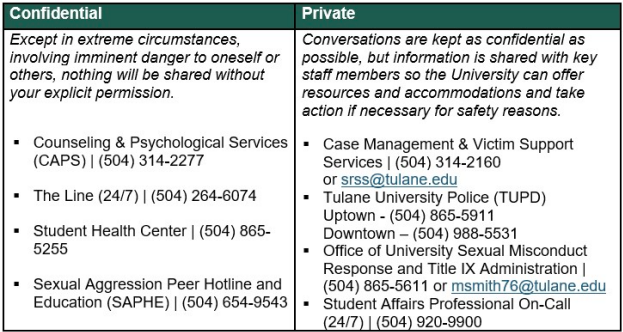
\includegraphics[width=1.0\textwidth]{TulaneTitleIX.jpg}
\end{figure}

\textbf{``Lauren's Promise'': I will listen and believe you if someone is threatening or harassing you.} Lauren McCluskey, a 21-year-old honors student athlete, was murdered on Oct. 22, 2018, by a man she briefly dated on the University of Utah campus. \textit{We must all take action to ensure that this never happens again.}

\section{Emergency Preparedness and Response}

\begin{figure}[H]
\centering
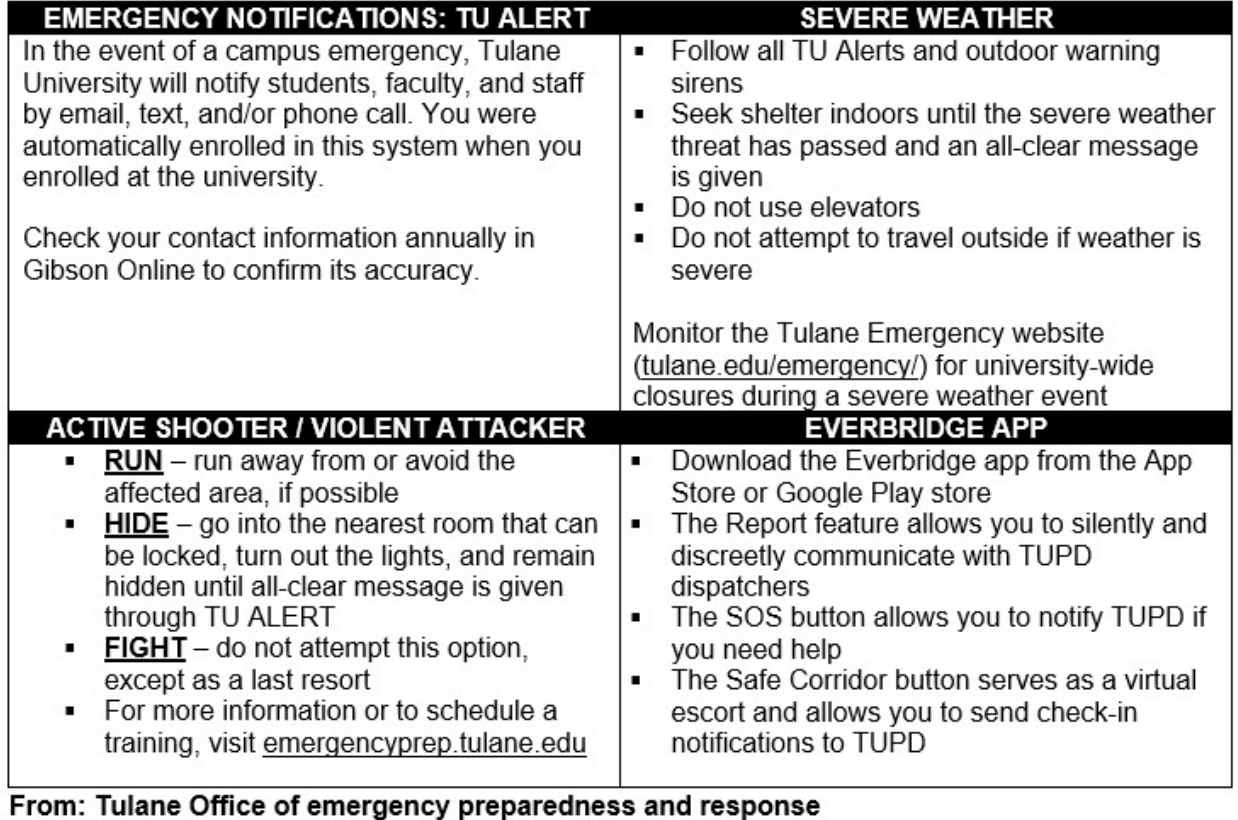
\includegraphics[width=1.0\textwidth]{TulaneEmergency2.jpg}
\end{figure}

\section{Class Schedule}

The schedule is tentative and is subject to change. 

\begin{table}[H]
\centering
\rowcolors{2}{gray!15}{white}
\begin{tabular}{@{}p{0.25\linewidth}p{0.65\linewidth}@{}}
\toprule
\textbf{Date (Spring 2024)} & \textbf{Class Activity} \\
\midrule
Jan. 16 (Tuesday) & Introduction to the Course \\
Jan. 18 (Thursday) & Geographical Definitions \& Scavenger Hunt + Finding data on data.census.gov \\
Jan. 23 (Tuesday) & Agglomeration, Clusters, and Cities \\
Jan. 25 (Thursday) & Practice Jigsaw - Economic Clusters \\
Jan. 30 (Tuesday) & Greenstone, Hornbeck, \& Moretti (2010) + Intro. to Diff-in-Diff \\
Feb. 1 (Thursday) & Reading Results Tables \\
Feb. 6 (Tuesday) & Econ. Development Incentives + Briefing Note + Briefing Note (Continued) \\
Feb. 8 (Thursday) & Quiz 1 \\
Feb. 13 (Tuesday) & Introduction to the Economics of Crime \\
Feb. 15 (Thursday) & Intro to Measuring the Effect of Police on Crime + Misc. \\
Feb. 20 (Tuesday) & Measuring the effect of police on crime + Measuring the effect of economic circumstances on crime \\
Feb. 22 (Thursday) & Economics Research on Gender-Based Violence - Jigsaw \\
Feb. 27 (Tuesday) & Manage COVID-19 and Gender-Based Violence \\
Mar. 5 (Tuesday) & Quiz 2 \\
Mar. 7 (Thursday) & Introduction to the Economics of Discrimination \\
Mar. 12 (Tuesday) & Racial Bias in the Criminal Justice System + Racial Bias in Policing + Racial Bias in Police Use of Force \\
Mar. 14 (Thursday) & Body Cameras, Pattern and Practice, and Other Policies to Prevent Racial Bias in Policing \\
Mar. 19 (Tuesday) & Racial Bias Group Briefing Note \\
Mar. 21 (Thursday) & Effect of Incarceration on Recidivism, Education, and Labor Market Outcomes and Ban the Box\\
\textbf{Mar. 23 (Saturday) to Mar. 31 (Sunday)} & \textbf{Spring Break (No Classes)} \\
Apr. 2 (Tuesday) & Quiz 3 \\
Apr. 4 (Thursday) & Housing Polices and Economic Theory and Housing Policies in Action - Metcalf (2018) \\
Apr. 9 (Tuesday) & Sexual Orientation Discrimination in Mortgages - Data Collection Demo and RA Job Information \\
Apr. 11 (Thursday) & Homelessness - Family Options Study \\
Apr. 16 (Tuesday) & Neighborhood Effects and Moving to Opportunity \\
Apr. 18 (Thursday) & Rent Control - Collecting Evidence \\
Apr. 23 (Tuesday) & Rent Control Briefing Note + Briefing Note (Continued) \\
Apr. 25 (Thursday) & Quiz 4 \\
Apr. 30 (Tuesday) & Course review study guide \\
\textbf{May 1 (Wednesday)} & \textbf{Last Day of Classes} \\

\end{tabular}
\caption{Spring 2024 Urban Economics Class Schedule}
\end{table}
  

%-------------------------------------------
% Begin bibliography
\newpage
\section{References: Readings on the Syllabus}
\def\refname{}
\bibliography{library}
\bibliographystyle{aea}

% End bibliography
%-------------------------------------------

\end{document}
